\documentclass[twocolumn]{article}
\usepackage{lmodern}
\usepackage{amssymb,amsmath}
\usepackage{ifxetex,ifluatex}
\usepackage{fixltx2e} % provides \textsubscript
\ifnum 0\ifxetex 1\fi\ifluatex 1\fi=0 % if pdftex
  \usepackage[T1]{fontenc}
  \usepackage[utf8]{inputenc}
\else % if luatex or xelatex
  \ifxetex
    \usepackage{mathspec}
  \else
    \usepackage{fontspec}
  \fi
  \defaultfontfeatures{Ligatures=TeX,Scale=MatchLowercase}
\fi
% use upquote if available, for straight quotes in verbatim environments
\IfFileExists{upquote.sty}{\usepackage{upquote}}{}
% use microtype if available
\IfFileExists{microtype.sty}{%
\usepackage[]{microtype}
\UseMicrotypeSet[protrusion]{basicmath} % disable protrusion for tt fonts
}{}
\PassOptionsToPackage{hyphens}{url} % url is loaded by hyperref
\usepackage[unicode=true]{hyperref}
\hypersetup{
            pdftitle={Using more LaTeX packages},
            pdfborder={0 0 0},
            breaklinks=true}
\urlstyle{same}  % don't use monospace font for urls
\usepackage[margin=1in]{geometry}
\usepackage{color}
\usepackage{fancyvrb}
\newcommand{\VerbBar}{|}
\newcommand{\VERB}{\Verb[commandchars=\\\{\}]}
\DefineVerbatimEnvironment{Highlighting}{Verbatim}{commandchars=\\\{\}}
% Add ',fontsize=\small' for more characters per line
\usepackage{framed}
\definecolor{shadecolor}{RGB}{248,248,248}
\newenvironment{Shaded}{\begin{snugshade}}{\end{snugshade}}
\newcommand{\KeywordTok}[1]{\textcolor[rgb]{0.13,0.29,0.53}{\textbf{#1}}}
\newcommand{\DataTypeTok}[1]{\textcolor[rgb]{0.13,0.29,0.53}{#1}}
\newcommand{\DecValTok}[1]{\textcolor[rgb]{0.00,0.00,0.81}{#1}}
\newcommand{\BaseNTok}[1]{\textcolor[rgb]{0.00,0.00,0.81}{#1}}
\newcommand{\FloatTok}[1]{\textcolor[rgb]{0.00,0.00,0.81}{#1}}
\newcommand{\ConstantTok}[1]{\textcolor[rgb]{0.00,0.00,0.00}{#1}}
\newcommand{\CharTok}[1]{\textcolor[rgb]{0.31,0.60,0.02}{#1}}
\newcommand{\SpecialCharTok}[1]{\textcolor[rgb]{0.00,0.00,0.00}{#1}}
\newcommand{\StringTok}[1]{\textcolor[rgb]{0.31,0.60,0.02}{#1}}
\newcommand{\VerbatimStringTok}[1]{\textcolor[rgb]{0.31,0.60,0.02}{#1}}
\newcommand{\SpecialStringTok}[1]{\textcolor[rgb]{0.31,0.60,0.02}{#1}}
\newcommand{\ImportTok}[1]{#1}
\newcommand{\CommentTok}[1]{\textcolor[rgb]{0.56,0.35,0.01}{\textit{#1}}}
\newcommand{\DocumentationTok}[1]{\textcolor[rgb]{0.56,0.35,0.01}{\textbf{\textit{#1}}}}
\newcommand{\AnnotationTok}[1]{\textcolor[rgb]{0.56,0.35,0.01}{\textbf{\textit{#1}}}}
\newcommand{\CommentVarTok}[1]{\textcolor[rgb]{0.56,0.35,0.01}{\textbf{\textit{#1}}}}
\newcommand{\OtherTok}[1]{\textcolor[rgb]{0.56,0.35,0.01}{#1}}
\newcommand{\FunctionTok}[1]{\textcolor[rgb]{0.00,0.00,0.00}{#1}}
\newcommand{\VariableTok}[1]{\textcolor[rgb]{0.00,0.00,0.00}{#1}}
\newcommand{\ControlFlowTok}[1]{\textcolor[rgb]{0.13,0.29,0.53}{\textbf{#1}}}
\newcommand{\OperatorTok}[1]{\textcolor[rgb]{0.81,0.36,0.00}{\textbf{#1}}}
\newcommand{\BuiltInTok}[1]{#1}
\newcommand{\ExtensionTok}[1]{#1}
\newcommand{\PreprocessorTok}[1]{\textcolor[rgb]{0.56,0.35,0.01}{\textit{#1}}}
\newcommand{\AttributeTok}[1]{\textcolor[rgb]{0.77,0.63,0.00}{#1}}
\newcommand{\RegionMarkerTok}[1]{#1}
\newcommand{\InformationTok}[1]{\textcolor[rgb]{0.56,0.35,0.01}{\textbf{\textit{#1}}}}
\newcommand{\WarningTok}[1]{\textcolor[rgb]{0.56,0.35,0.01}{\textbf{\textit{#1}}}}
\newcommand{\AlertTok}[1]{\textcolor[rgb]{0.94,0.16,0.16}{#1}}
\newcommand{\ErrorTok}[1]{\textcolor[rgb]{0.64,0.00,0.00}{\textbf{#1}}}
\newcommand{\NormalTok}[1]{#1}
\usepackage{graphicx,grffile}
\makeatletter
\def\maxwidth{\ifdim\Gin@nat@width>\linewidth\linewidth\else\Gin@nat@width\fi}
\def\maxheight{\ifdim\Gin@nat@height>\textheight\textheight\else\Gin@nat@height\fi}
\makeatother
% Scale images if necessary, so that they will not overflow the page
% margins by default, and it is still possible to overwrite the defaults
% using explicit options in \includegraphics[width, height, ...]{}
\setkeys{Gin}{width=\maxwidth,height=\maxheight,keepaspectratio}
\IfFileExists{parskip.sty}{%
\usepackage{parskip}
}{% else
\setlength{\parindent}{0pt}
\setlength{\parskip}{6pt plus 2pt minus 1pt}
}
\setlength{\emergencystretch}{3em}  % prevent overfull lines
\providecommand{\tightlist}{%
  \setlength{\itemsep}{0pt}\setlength{\parskip}{0pt}}
\setcounter{secnumdepth}{0}
% Redefines (sub)paragraphs to behave more like sections
\ifx\paragraph\undefined\else
\let\oldparagraph\paragraph
\renewcommand{\paragraph}[1]{\oldparagraph{#1}\mbox{}}
\fi
\ifx\subparagraph\undefined\else
\let\oldsubparagraph\subparagraph
\renewcommand{\subparagraph}[1]{\oldsubparagraph{#1}\mbox{}}
\fi

% set default figure placement to htbp
\makeatletter
\def\fps@figure{htbp}
\makeatother

\usepackage{amsmath}
\usepackage{threeparttable}

\title{Using more LaTeX packages}
\author{}
\date{\vspace{-2.5em}}

\begin{document}
\maketitle

\section{Conceptos básicos de
estadística}\label{conceptos-buxe1sicos-de-estaduxedstica}

\section{Muestreo}\label{muestreo}

\subsection{Muestreo probabilistico: misma probabilidad para todos los
elementos de ser seleccionados en la poblacion
muestral.}\label{muestreo-probabilistico-misma-probabilidad-para-todos-los-elementos-de-ser-seleccionados-en-la-poblacion-muestral.}

\subsection{Muestreo no probabilistico: Seleccion arbitraria
seleccionada por el
investigador}\label{muestreo-no-probabilistico-seleccion-arbitraria-seleccionada-por-el-investigador}

\section{Población (universo o
colectivo)}\label{poblaciuxf3n-universo-o-colectivo}

Es el conjunto total de ELEMENTOS de la misma naturaleza cualquera que
sea, que son de interés para un problema dado

\begin{itemize}
\tightlist
\item
  N = Representación de el tamaño de la población
\end{itemize}

\section{muestra}\label{muestra}

\subsection{Variable aleatoria:}\label{variable-aleatoria}

Son fenómenos o características de los elementos de la población.

Función de valor real que tiene como dominio el espacio muestral de un
experimento aleatorio.

Variables sobre las cuales tenemos un grado de icertidumbre respecto a
los valores que puede tomar

\subsection{Datos}\label{datos}

Son los resultados observados de las variables aleatorias (Cuando se
hace una medición)

\subsection{Parámetro}\label{paruxe1metro}

Es la medición global de cualesquer característica de los elementos de
la población.

Es un valor teórico asociado a la población.

\subsubsection{Ejemplos}\label{ejemplos}

\paragraph{Población: Los niños y niñas de 0 a 5 años de edad
localozados en
Bogotá}\label{poblaciuxf3n-los-niuxf1os-y-niuxf1as-de-0-a-5-auxf1os-de-edad-localozados-en-bogotuxe1}

\paragraph{Variables: género, edad, peso, talla, estrato, localidad,
fecha, lugar de
nacimiento..}\label{variables-guxe9nero-edad-peso-talla-estrato-localidad-fecha-lugar-de-nacimiento..}

\paragraph{Parámetros: IMC}\label{paruxe1metros-imc}

\section{Clasificacion de variables}\label{clasificacion-de-variables}

\subsection{Cualitativas
(categóricas)}\label{cualitativas-categuxf3ricas}

\subsection{Cuantitativas}\label{cuantitativas}

Los valores de las observacione so niméricas y en conseciencia,
ordenables.

\subsubsection{Discreta}\label{discreta}

Recorridos finitos numerables sin tomar valores intermedios
e.g.~conteos.

\subsubsection{Continua}\label{continua}

Recorridos infinitos no numerables e.g.~la distribución normal

\section{Escalas de medición}\label{escalas-de-mediciuxf3n}

\subsection{Cualitativas}\label{cualitativas}

\subsubsection{Nominales: Clasificación de objetos o fenómenos mediante
símbolos o signos (No hay orden o dirección).
e.g.}\label{nominales-clasificaciuxf3n-de-objetos-o-fenuxf3menos-mediante-suxedmbolos-o-signos-no-hay-orden-o-direcciuxf3n.-e.g.}

\begin{itemize}
\tightlist
\item
  Nombre
\item
  Número de la cédula
\item
  Tipo de sangre
\item
  Color de los ojos
\item
  Número de camiseta de los jugadores
\end{itemize}

Los números en la lista anterior no pueden ser sometidos a operaciones
matemáticas

\subsubsection{Ordinales}\label{ordinales}

Categorías ordenadas (Rangos, órdenes, escalamientos)

\begin{itemize}
\tightlist
\item
  Sabor de un yogurt
\end{itemize}

\subsection{Cuantitativas}\label{cuantitativas-1}

\subsubsection{Intervalo}\label{intervalo}

Los datos medidos en una escala orrdinal para los cuales pueden
clasificarse las distancias entre valores pero no existe un cero
absoluto o no exista ausencia total de la característica

\begin{itemize}
\tightlist
\item
  Temperatura: a 0°C no deja de existir la temperatura
\item
  Notas: se corre la escala e inicia desde 3.
\end{itemize}

\subsubsection{Razón}\label{razuxf3n}

Tiene todas las características de un intervalo, y además tiene un cero
absoluto

\section{Resumen y descripción de datos de una
variable}\label{resumen-y-descripciuxf3n-de-datos-de-una-variable}

Datos en bruto en forma de listas (o bases no son fáciles de usar para
tomar decisiones)

\begin{itemize}
\tightlist
\item
  Se necesita algún tipo de organización
\end{itemize}

Para esto podemos utilizar gráficos de barras, graficos de torta, o
tablas de frecuencias.

\section{Como agrupar los datos:
Sturgues}\label{como-agrupar-los-datos-sturgues}

Si n no es demasiado grande, intervalos = \(\sqrt{n}\)

En caso contrario:

\begin{align}
k = 1 + 3.322 log(n)
\end{align}

k = intervalos de clase

Para la longitud de los intervalos:

\begin{align}
L = \frac{Dato \; mayor - Dato \; menor}{n}
\end{align}

\begin{itemize}
\tightlist
\item
  A menudo es prueba y error
\end{itemize}

\section{Tipos de frecuencias}\label{tipos-de-frecuencias}

\begin{itemize}
\tightlist
\item
  Absoluta: Conteo de observaciones que cae en cada intervalo.
\item
  Relativa: \(\frac{Absoluta}{n}\).
\item
  Acumulada: Suma de las frecuencias absolutas
\item
  Relativa acumulada: Suma de las frecuencias relativas.
\end{itemize}

\section{Caracteristicas a revisar de las
distribuciones}\label{caracteristicas-a-revisar-de-las-distribuciones}

\begin{itemize}
\tightlist
\item
  Distribucion
\item
  Localizacion (sesgo)
\item
  Dispersion
\end{itemize}

\section{Medidas de localización}\label{medidas-de-localizaciuxf3n}

\subsection{Media aritmética:}\label{media-aritmuxe9tica}

Si \(x_1, x_2, x_3,...x_n\) es una muestra de una poblacion de tamaño N
entonces la media es N

\subsubsection{Media poblacional}\label{media-poblacional}

\begin{align}
\mu = \frac{\sum_{i=1}^n x_i}{N}
\end{align}

\subsubsection{Estimador muestral}\label{estimador-muestral}

\begin{align}
\bar{x} = \frac{\sum_{i=1}^n x_i}{n}
\end{align}

Caracteristicas:

\begin{itemize}
\tightlist
\item
  Es facil de obtener
\item
  Medida no robusta: Afectada por valores extremos o datos atípicos.
\end{itemize}

\subsubsection{Propiedades de la media
aritmetica:}\label{propiedades-de-la-media-aritmetica}

Si \(x_1, x_2, x_3,...x_n\) es una muestra de una poblacion de tamaño N
entonces la media es N, entonces

\begin{align}
\sum_{i=1}^n x_i = x_1 + x_2 + x_3 + \cdot \cdot \cdot + x_n
\end{align}

Si \(x_i = c\) y a su vez c es constante, entonces

\begin{align}
\sum_{i=1}^ n x_i = \sum_{i=1} c = c + c + c +  \cdot \cdot \cdot 
\end{align}

Entonces

\begin{align}
\sum_{i=1}^n x_i = nc
\end{align}

\begin{itemize}
\tightlist
\item
  \emph{Ejemplo:}
\end{itemize}

\begin{align}
\sum_{i=1}^5 2 = 2 + 2 + 2 + 2 + 2
\end{align}

Si c es una constante que multiplica las observaciones:

\begin{align}
\sum_{i=1}^n c x_i = c \sum_{i=1}^n x_i
\end{align}

\begin{align}
\sum_{i=1}^n c x_i = c \cdot x_1 + c \cdot x_2 + c \cdot x_3 + \cdot \cdot \cdot + c \cdot x_n
\end{align}

\begin{align}
\sum_{i=1}^n c x_i = c \; (x_1 +   x_2 +  x_3 + \cdot \cdot \cdot +   x_n)
\end{align}

\begin{align}
\sum_{i=1}^n c x_i = c \sum_{i=1}^n x_i
\end{align}

Si \(x_1, x_2, x_3,...x_n\) y \(y_1, y_2, y_3,...y_n\) son sucesiones de
numeros;

\begin{align}
\sum_{i=1}^n (x_i + y_i) =  \sum_{i=1}^n x_i + \sum_{i=1}^n y_i
\end{align}

\begin{align}
\sum_{i=1}^n (x_i + y_i) =  (x_1 + y_1) 
+ (x_2 + y_2) + (x_3 + y_3) + \cdot \cdot \cdot + (x_n + y_n)
\end{align}

\begin{align}
\sum_{i=1}^n (x_i + y_i) =  (x_1 + x_2 + \cdot \cdot \cdot + x_n ) + (y_1 + y_2 + \cdot \cdot \cdot + y_n )
\end{align}

\begin{align}
\sum_{i=1}^n (x_i + y_i) =  \sum_{i=1}^n x_i + \sum_{i=1}^n y_i
\end{align}

Si \(x_1, x_2, x_3,...x_n\) y \(y_1, y_2, y_3,...y_n\) son sucesiones de
numeros;

\begin{align}
\sum_{i=1}^n (x_i - y_i) =  \sum_{i=1}^n x_i - \sum_{i=1}^n y_i
\end{align}

\begin{enumerate}
\def\labelenumi{\arabic{enumi}.}
\setcounter{enumi}{4}
\item
\end{enumerate}

\begin{align}
\sum_{i=1}^n (x_i - \bar{x}) = 0
\end{align}

\begin{align}
\sum_{i=1}^n (x_i - \bar{x}) =  \sum_{i=1}^n x_i - \sum_{i=1}^n \bar{x}
\end{align}

\begin{align}
 \sum_{i=1}^n (x_i - \bar{x}) = \frac{n}{n} \sum_{i=1}^n x_i - n \bar{x}
\end{align}

\begin{align}
 \sum_{i=1}^n (x_i - \bar{x}) = n \bar{x} - n \bar{x}
\end{align}

\begin{align}
 \sum_{i=1}^n (x_i - \bar{x}) = 0
\end{align}

\begin{enumerate}
\def\labelenumi{\arabic{enumi}.}
\setcounter{enumi}{5}
\item
\end{enumerate}

promedio de y en funcion de promedio de x en regresion lineal simple

Si \(y_i = a + b x_i\) siendo a y b constante

\begin{align}
\bar{y} = a + b \bar{x}
\end{align}

En efecto:

\begin{align}
\sum_{i= 1}^n y_i = \sum_{i=1}^n (a + b x_i)
\end{align}

\begin{align}
\sum_{i= 1}^n y_i = \sum_{i=1}^n a + \sum_{i=1}^n b x_i
\end{align}

\begin{align}
\sum_{i= 1}^n y_i = na + b \sum_{i=1}^n  x_i
\end{align}

\begin{align}
\frac{\sum_{i= 1}^n y_i}{n} = \frac{na}{n} +b \frac{ \sum_{i=1}^n  x_i}{n}
\end{align}

\begin{align}
\bar{y} = a + b \bar{x} 
\end{align}

\subsection{La mediana}\label{la-mediana}

Es el valor central (es el dato de la variable que esta en el centro de
la misma). Deja por encima y por debajo mitad y mitad de las
observaciones.

\subsubsection{Calculo de la mediana}\label{calculo-de-la-mediana}

Depende si el conjunto es par o impar:

Si\(x_1, x_2, x_3,...x_n\) Son los valores ordenados en una muestra de
una poblacion de tamaño N:

\(\hat{x} = \frac{x_{n/2}+x_{n+1/2} }{2}\) si n es par

\(\hat{x} = x_{n=1/2}\) si n es impar

Es un estimador robusto, no se ve afectado por valores extremos

\subsubsection{Ejemplo}\label{ejemplo}

Edad de ninos

\begin{Shaded}
\begin{Highlighting}[]
\NormalTok{x1 <-}\StringTok{ }\KeywordTok{c}\NormalTok{(}\DecValTok{6}\NormalTok{,}\DecValTok{7}\NormalTok{,}\DecValTok{8}\NormalTok{,}\DecValTok{9}\NormalTok{,}\DecValTok{10}\NormalTok{)}
\end{Highlighting}
\end{Shaded}

n es impar, entonces \(\hat{x} = x_{n+1/2}=x_{6/2} = x_3 = 8\)

De la muestra analizada la mitad de los ninos tienen entre 6 y 8 años, y
la otra mitad entre 8 y 10 años.

\section{Moda}\label{moda}

\begin{itemize}
\tightlist
\item
  El valor que más se repite
\item
  Usada para valores numéricos o categóricos
\end{itemize}

e.g.~Cual es el color más frecuente en los ojos.

\section{Medidas de dispersión o
variación}\label{medidas-de-dispersiuxf3n-o-variaciuxf3n}

\subsection{Varianza}\label{varianza}

Uno de los problemas es que la unidad de medida queda al cuadrado,
e.g.~si se miden cm, la varianza tiene unidades de \(cm^2\):

\begin{itemize}
\tightlist
\item
  Varianza poblacional:
\end{itemize}

\begin{align}
\sigma^2= \frac{\sum_{i=1}^N (x_i - \mu)^2}{N}
\end{align}

\begin{itemize}
\tightlist
\item
  Varianza muestral:
\end{itemize}

\begin{align}
s^2= \frac{\sum_{i=1}^n (x_i - \bar{x})^2}{n-1}
\end{align}

\begin{align}
s^2 = \sum_{i=1}^n \frac{x_i^2 - 2x_i\bar{x}+ \bar{x}^2}{n-1}
\end{align}

\begin{align}
s^2 =  \frac{\sum_{i=1}^n x_i^2 - 2\bar{x}\sum_{i=1}^n x_i+ n\bar{x}^2}{n-1}
\end{align}

\begin{align}
s^2 =  \frac{\sum_{i=1}^n x_i^2 - 2\bar{x} \frac{n}{n}\sum_{i=1}^n x_i + n\bar{x}^2}{n-1}
\end{align}

\begin{align}
s^2 =  \frac{\sum_{i=1}^n x_i^2 - 2\bar{x} n \bar{x} + n\bar{x}^2}{n-1}
\end{align}

\begin{align}
s^2 =  \frac{\sum_{i=1}^n x_i^2 - 2 n \bar{x}^2 + n\bar{x}^2}{n-1}
\end{align}

\begin{align}
s^2 =  \frac{\sum_{i=1}^n x_i^2 - n \bar{x}^2 }{n-1}
\end{align}

\begin{align}
s^2 =  \frac{\sum_{i=1}^n x_i^2}{n-1} -\frac{ n \bar{x}^2 }{n-1}
\end{align}

\begin{align}
s^2 =  \frac{\sum_{i=1}^n x_i^2}{n-1} -\frac{ n }{n-1}
\left( \frac{\sum_{i=1}^n x_i}{n} \right)^2
\end{align}

\begin{align}
s^2 =  \frac{\sum_{i=1}^n x_i^2}{n-1} -\frac{ 1 }{n-1}
 \frac{\left(\sum_{i=1}^n x_i\right)^2}{n} 
\end{align}

En algunos casos puede ser más conveniente calcular la varianza de esta
forma.

\subsection{Coeficiente de variación}\label{coeficiente-de-variaciuxf3n}

\(CV = \frac{s}{\hat{x}} \cdot 100 \%\)

Si CV es igual o menor a \(5 \%\) hay homogeneidad

si esta entre \(5\%\) y \(20\%\) los datos son medianamente homogeneos

Si CV mayor a 20\% hay heterogeneidad\\
\#\# Rango

medida no robusta, si hay datos atipicos se ve muy afectado

\subsection{rango intercuartilico}\label{rango-intercuartilico}

boxplot

\section{Cuartiles}\label{cuartiles}

Se divide en cuatro partes porcentiales el conjunto de observaciones.

Se calcula de la sigueinte manera.

Se ordena la muestra y se toma la posicion que corresponde.

\(Q_k = k \cdot \frac{n}{4} \; k =1,2,3\)

\subsection{Deciles}\label{deciles}

Se divide en diez partes porcertialmente iguales

\(D_k = \frac{n}{10} \; 1,2,3,...,9\)

\subsection{Percentiles}\label{percentiles}

es mas detallado, nos da mas acceso a distintos puntos de la
distribucion

\(P_k = \frac{n}{100} \; 1,2,3,...,99\)

\section{Coeficientes de asimetría de
Fisher}\label{coeficientes-de-asimetruxeda-de-fisher}

Permite interpretar la forma de la distribución, respecto a ser o no
asimétrica

\section{Coeficiente de curtosis}\label{coeficiente-de-curtosis}

Mide el grado de aplastamiento o apuntamiento de la gráfica de la
distribución.

\section{Otras medidas de
centralización}\label{otras-medidas-de-centralizaciuxf3n}

\subsection{Desviacion media absoluta}\label{desviacion-media-absoluta}

\begin{align}
DM = \frac{\sum_{i = 1}^n |x_i - \bar{x}|}{n}
\end{align}

\subsection{Media ponderada}\label{media-ponderada}

\subsection{Media geometrica}\label{media-geometrica}

\subsection{Media armonica}\label{media-armonica}

Sirve en diseño de experimentos par aproximar el numero de replicas en
todo el expermineto cuando el diseño es desbalanceado.

\section{Ejemplo en excel}\label{ejemplo-en-excel}

Tabla de pesos de mujeres en una empresa

\begin{enumerate}
\def\labelenumi{\arabic{enumi}.}
\tightlist
\item
  construcción de la tabla de frecuencias
\end{enumerate}

\begin{itemize}
\tightlist
\item
  Definición de los intervalos: podemos utilizar la siguiente ecuación:
\end{itemize}

\begin{align}
k = 1 + 3.322 log_{10} (n)
\end{align}

Para esta muestra de 50 pesos de mujeres:

\begin{align}
k = 1 + 3.322 log_{10} (50)
\end{align}

\begin{align}
k = 6.6 \approx 7
\end{align}

Vamos a usar 7 intervalos, para saber la longitud dividimos el rango en
el numero de intervalos.

Para hallar el rango podemos importar los datos a R:

\begin{Shaded}
\begin{Highlighting}[]
\NormalTok{tablaPesos <-}\StringTok{ }\KeywordTok{read.table}\NormalTok{(}\StringTok{"TABLAPESOS.txt"}\NormalTok{, }\DataTypeTok{header =}\NormalTok{ T)}
\end{Highlighting}
\end{Shaded}

Y luego preguntar sobre el valor maximo y el minimo:

\begin{Shaded}
\begin{Highlighting}[]
\KeywordTok{max}\NormalTok{(tablaPesos)}
\end{Highlighting}
\end{Shaded}

\begin{verbatim}
## [1] 72
\end{verbatim}

\begin{Shaded}
\begin{Highlighting}[]
\KeywordTok{min}\NormalTok{(tablaPesos)}
\end{Highlighting}
\end{Shaded}

\begin{verbatim}
## [1] 53
\end{verbatim}

Podemos entonces calcular la longitud de cada intervalo:

\begin{Shaded}
\begin{Highlighting}[]
\NormalTok{(}\KeywordTok{max}\NormalTok{(tablaPesos)}\OperatorTok{-}\KeywordTok{min}\NormalTok{(tablaPesos))}\OperatorTok{/}\DecValTok{7}
\end{Highlighting}
\end{Shaded}

\begin{verbatim}
## [1] 2.714286
\end{verbatim}

Obtenemos una longitud de intervalo de \(2.71 \approx 3\)

Los intervalos entonces serían:

\begin{verbatim}
##   intervalo valores
## 1         1   53 55
## 2         2   56 58
## 3         3   59 61
## 4         4   62 64
## 5         5   65 67
## 6         6   68 70
## 7         7   71 73
\end{verbatim}

En excel:

\begin{itemize}
\tightlist
\item
  Usamos los limites superiores de los intervalos

  \begin{itemize}
  \tightlist
  \item
    Datos, analisis de datos, histograma, aceptar, seleccionar rango de
    entrada, rango de clases son los limites superiores. Al hacer esto,
    excel genera una tabla como la siguiente:
  \end{itemize}
\end{itemize}

\begin{figure}
\centering
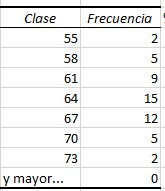
\includegraphics{./img/frecuenciasExcel.jpg}
\caption{tabla de frecuencias en excel}
\end{figure}

Luego, a partir de esta tabla podemos calcular todas las frecuencias, la
frecuencia absoluta (\(f_i\)), recuencia relativa (\(f_r\)), la
frecuencia absoluta acumulada (\(F_i\)) y la frecuencia relativa
acumulada (\(F_r\)):

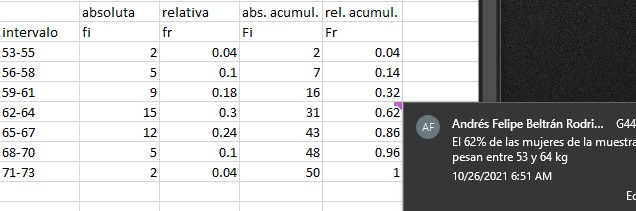
\includegraphics{./img/tablaDeFrecuencias.jpg} Luego a partir de esta
tabla de frecuencias, utilizando las columnas de intervalo y \% de
frecuencia podemos construir un histograma como el siguiente:

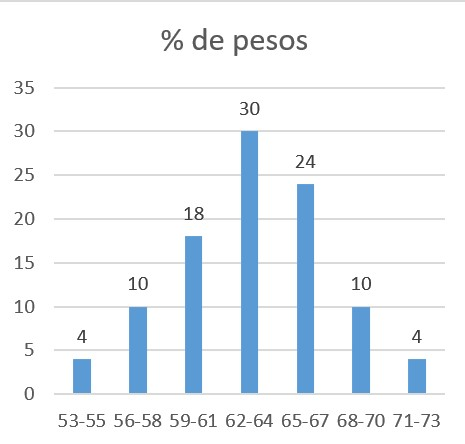
\includegraphics{./img/histogramaPorcentajes.jpg} Para hacer una
operación análoga en R podemos crear los intervalos de la siguiente
manera:

\begin{Shaded}
\begin{Highlighting}[]
\NormalTok{mins <-}\StringTok{ }\KeywordTok{seq}\NormalTok{(}\DecValTok{53}\NormalTok{,}\DecValTok{71}\NormalTok{, }\DataTypeTok{by =} \DecValTok{3}\NormalTok{)}
\NormalTok{maxs <-}\StringTok{ }\KeywordTok{seq}\NormalTok{(}\DecValTok{55}\NormalTok{,}\DecValTok{73}\NormalTok{, }\DataTypeTok{by =} \DecValTok{3}\NormalTok{)}
\end{Highlighting}
\end{Shaded}

Luego, podemos juntar las dos columnas de limites inferiores y
superiores de intervalo en la tabla \texttt{TDF}:

\begin{Shaded}
\begin{Highlighting}[]
\NormalTok{TDF <-}\StringTok{ }\KeywordTok{data.frame}\NormalTok{(}\DataTypeTok{min =}\NormalTok{ mins,}
                                 \DataTypeTok{max =}\NormalTok{ maxs )}
\NormalTok{TDF}
\end{Highlighting}
\end{Shaded}

\begin{verbatim}
##   min max
## 1  53  55
## 2  56  58
## 3  59  61
## 4  62  64
## 5  65  67
## 6  68  70
## 7  71  73
\end{verbatim}

Luego podemos iterar a lo largo de las filas de
\texttt{tablasDefrecuencias} buscando cuantos elementos de
\texttt{tablaDePesos} están dentro del intervalo definido por cada fila:

\begin{Shaded}
\begin{Highlighting}[]
\ControlFlowTok{for}\NormalTok{(i }\ControlFlowTok{in} \DecValTok{1}\OperatorTok{:}\KeywordTok{nrow}\NormalTok{(TDF)) \{}
\NormalTok{  TDF}\OperatorTok{$}\NormalTok{Freq[i] <-}
\StringTok{      }\KeywordTok{length}\NormalTok{(}
          \KeywordTok{which}\NormalTok{(}
\NormalTok{mins[i] }\OperatorTok{<=}\StringTok{  }\NormalTok{tablaPesos }\OperatorTok{&}\StringTok{ }\NormalTok{tablaPesos}\OperatorTok{<=}\StringTok{ }\NormalTok{maxs[i]))}
\NormalTok{\}}
\end{Highlighting}
\end{Shaded}

Podemos luego calcular la frecuencia relativa dividiendo por el total de
observaciones:

\begin{Shaded}
\begin{Highlighting}[]
\NormalTok{TDF}\OperatorTok{$}\NormalTok{fr <-TDF}\OperatorTok{$}\NormalTok{Freq}\OperatorTok{/}
\StringTok{    }\KeywordTok{sum}\NormalTok{(TDF}\OperatorTok{$}\NormalTok{Freq)}

\NormalTok{TDF}
\end{Highlighting}
\end{Shaded}

\begin{verbatim}
##   min max Freq   fr
## 1  53  55    2 0.04
## 2  56  58    5 0.10
## 3  59  61    9 0.18
## 4  62  64   15 0.30
## 5  65  67   12 0.24
## 6  68  70    5 0.10
## 7  71  73    2 0.04
\end{verbatim}

Luego podemos calcular la frecuencia absoluta y relativa acumuladas para
cada intervalo de manera ascendiente:

\begin{Shaded}
\begin{Highlighting}[]
\ControlFlowTok{for}\NormalTok{(i }\ControlFlowTok{in} \DecValTok{1}\OperatorTok{:}\KeywordTok{nrow}\NormalTok{(TDF))\{}

\NormalTok{TDF}\OperatorTok{$}\NormalTok{Fi[i] <-}\StringTok{ }\KeywordTok{sum}\NormalTok{(TDF}\OperatorTok{$}\NormalTok{Freq[}\DecValTok{1}\OperatorTok{:}\NormalTok{i])}

\NormalTok{\}}
\end{Highlighting}
\end{Shaded}

Podemos hacer lo mismo para la frecuencia relativa acumulada (\(F_r\)):

\begin{Shaded}
\begin{Highlighting}[]
\ControlFlowTok{for}\NormalTok{(i }\ControlFlowTok{in} \DecValTok{1}\OperatorTok{:}\KeywordTok{nrow}\NormalTok{(TDF))\{}

\NormalTok{TDF}\OperatorTok{$}\NormalTok{Fr[i] <-}\StringTok{ }\KeywordTok{sum}\NormalTok{(TDF}\OperatorTok{$}\NormalTok{fr[}\DecValTok{1}\OperatorTok{:}\NormalTok{i])}

\NormalTok{\}}
\end{Highlighting}
\end{Shaded}

Una vez tenemos la tabla de frecuencias completa, podemos hacer la
gráfica de frecuencias porcentuales:

\begin{Shaded}
\begin{Highlighting}[]
\KeywordTok{library}\NormalTok{(ggplot2)}
\end{Highlighting}
\end{Shaded}

\begin{verbatim}
## Warning: package 'ggplot2' was built under R version 4.0.3
\end{verbatim}

\begin{Shaded}
\begin{Highlighting}[]
\NormalTok{intervalos <-}\StringTok{ }\KeywordTok{factor}\NormalTok{(}\KeywordTok{paste}\NormalTok{(TDF}\OperatorTok{$}\NormalTok{min,}\StringTok{'-'}\NormalTok{,TDF}\OperatorTok{$}\NormalTok{max))}

\KeywordTok{ggplot}\NormalTok{(TDF,}
       \KeywordTok{aes}\NormalTok{(}\DataTypeTok{x =}\NormalTok{ intervalos,}
           \DataTypeTok{y =}\NormalTok{ fr}\OperatorTok{*}\DecValTok{100}\NormalTok{,}
           \DataTypeTok{fill=}\NormalTok{intervalos,}
           \DataTypeTok{label =} \KeywordTok{round}\NormalTok{(fr}\OperatorTok{*}\DecValTok{100}\NormalTok{,}\DecValTok{2}\NormalTok{)}
\NormalTok{           )}
\NormalTok{       ) }\OperatorTok{+}
\StringTok{    }\KeywordTok{geom_bar}\NormalTok{(}\DataTypeTok{stat=}\StringTok{"identity"}\NormalTok{) }\OperatorTok{+}
\StringTok{  }\KeywordTok{xlab}\NormalTok{(}\StringTok{"intervalo"}\NormalTok{) }\OperatorTok{+}
\StringTok{    }\KeywordTok{ylab}\NormalTok{(}\StringTok{'% frecuencia relativa'}\NormalTok{)}\OperatorTok{+}
\StringTok{  }\KeywordTok{geom_label}\NormalTok{(}\KeywordTok{aes}\NormalTok{(}\DataTypeTok{fill =}\NormalTok{ intervalos),}
             \DataTypeTok{colour =} \StringTok{"white"}\NormalTok{,}
             \DataTypeTok{fontface =} \StringTok{"italic"}\NormalTok{)}
\end{Highlighting}
\end{Shaded}

\includegraphics{ConceptosBasicosDeEstadistica_files/figure-latex/unnamed-chunk-11-1.pdf}

\section{Calculo de medidas
descriptivas}\label{calculo-de-medidas-descriptivas}

\begin{Shaded}
\begin{Highlighting}[]
\KeywordTok{mean}\NormalTok{(tablaPesos}\OperatorTok{$}\NormalTok{pesos)}
\end{Highlighting}
\end{Shaded}

\begin{verbatim}
## [1] 63.2
\end{verbatim}

\begin{Shaded}
\begin{Highlighting}[]
\KeywordTok{quantile}\NormalTok{(tablaPesos}\OperatorTok{$}\NormalTok{pesos)}
\end{Highlighting}
\end{Shaded}

\begin{verbatim}
##   0%  25%  50%  75% 100% 
## 53.0 61.0 63.5 66.0 72.0
\end{verbatim}

El 75\% de las mujeres pesan entre 53 y 66 kg. El 25\% restante pesa
entre 66 kg y 72 kg

\begin{itemize}
\item
  la varianza: Es importante calcular la varianza muestral y no la
  varianza poblacional, dado que no se puede saber la poblacional
  (\(\sigma^2\)) si no su estimador (\(s^2\)).
\item
  Algunos paquetes hacen calculos con la varianza poblacional
\end{itemize}

En R: `The denominator n - 1 is used which gives an unbiased estimator
of the (co)variance for i.i.d. observations.'

\begin{Shaded}
\begin{Highlighting}[]
\KeywordTok{var}\NormalTok{(tablaPesos}\OperatorTok{$}\NormalTok{pesos)}
\end{Highlighting}
\end{Shaded}

\begin{verbatim}
## [1] 17.10204
\end{verbatim}

Para calcular la varianza poblacional:

\begin{Shaded}
\begin{Highlighting}[]
\NormalTok{pesos <-}\StringTok{ }\NormalTok{tablaPesos}\OperatorTok{$}\NormalTok{pesos}
\KeywordTok{sum}\NormalTok{((pesos }\OperatorTok{-}\StringTok{ }\KeywordTok{mean}\NormalTok{(pesos))}\OperatorTok{^}\DecValTok{2}\NormalTok{)}\OperatorTok{/}\KeywordTok{length}\NormalTok{(pesos)}
\end{Highlighting}
\end{Shaded}

\begin{verbatim}
## [1] 16.76
\end{verbatim}

para el calculo de la desviacion estandar:

\begin{Shaded}
\begin{Highlighting}[]
\KeywordTok{sd}\NormalTok{(pesos)}
\end{Highlighting}
\end{Shaded}

\begin{verbatim}
## [1] 4.135461
\end{verbatim}

\begin{Shaded}
\begin{Highlighting}[]
\KeywordTok{sqrt}\NormalTok{(}\KeywordTok{var}\NormalTok{(pesos))}
\end{Highlighting}
\end{Shaded}

\begin{verbatim}
## [1] 4.135461
\end{verbatim}

Interpretación:

Varianza: Tiene unidades al cuadrado. Tendriamos que tener otro grupo de
comparación, con una medición similar.

Desviacion estandar: la desviacion de las observaciones respecto al
promedio es de 4.14 unidades de masa (kg).

Para calcular otros estadísticos descriptivos podemos utilizar en excel:

\begin{itemize}
\tightlist
\item
  Datos \textgreater{} Análisis de datos \textgreater{} Estadística
  descriptiva \textgreater{} Se selecciona rango de entrada y de salida.
\end{itemize}

Se obtiene la siguiente tabla:

\begin{figure}
\centering
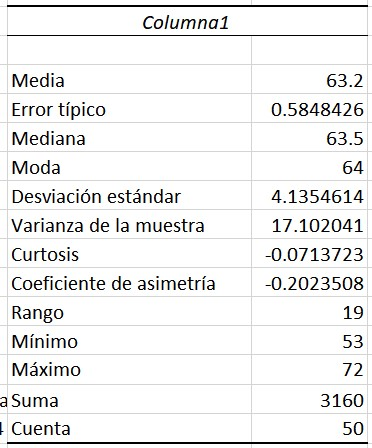
\includegraphics{./img/EstadisticaDescriptiva.jpg}
\caption{Cuadro de estadística descriptiva en excel}
\end{figure}

Dentro de esta tabla está el error típico

\subsection{Error típico - error
estándar}\label{error-tuxedpico---error-estuxe1ndar}

\begin{align}
\frac{s}{\sqrt(n)}
\end{align}

En este caso:

\begin{Shaded}
\begin{Highlighting}[]
\KeywordTok{sd}\NormalTok{(pesos)}\OperatorTok{/}\KeywordTok{sqrt}\NormalTok{(}\DecValTok{50}\NormalTok{)}
\end{Highlighting}
\end{Shaded}

\begin{verbatim}
## [1] 0.5848426
\end{verbatim}

Se utiliza para inferencia, para intervalos de confianza. En diseño de
experimentos sirve para el cálculo de tamaño de muestra. Se espera que
no aumente el número de réplicas si no disminuye lo suficiente el error
típico.

\begin{Shaded}
\begin{Highlighting}[]
\KeywordTok{library}\NormalTok{(e1071)}
\end{Highlighting}
\end{Shaded}

\begin{verbatim}
## Warning: package 'e1071' was built under R version 4.0.5
\end{verbatim}

\begin{Shaded}
\begin{Highlighting}[]
\KeywordTok{kurtosis}\NormalTok{(pesos)}
\end{Highlighting}
\end{Shaded}

\begin{verbatim}
## [1] -0.2936688
\end{verbatim}

\begin{Shaded}
\begin{Highlighting}[]
\KeywordTok{skewness}\NormalTok{(pesos)}
\end{Highlighting}
\end{Shaded}

\begin{verbatim}
## [1] -0.1903716
\end{verbatim}

La distribucion de pesos tiene una curtosis \(<3\), lo cual indica que
es mas aplanada que una distribucion normal, o tiene hombros más
pesados.

Además, tiene un coeficiende de asimetría cercano a cero, lo cual indica
un ligero sesgo con cola hacia valores menores de peso.

\begin{Shaded}
\begin{Highlighting}[]
\KeywordTok{range}\NormalTok{(pesos)}
\end{Highlighting}
\end{Shaded}

\begin{verbatim}
## [1] 53 72
\end{verbatim}

\begin{Shaded}
\begin{Highlighting}[]
\KeywordTok{range}\NormalTok{(pesos)[}\DecValTok{2}\NormalTok{] }\OperatorTok{-}\StringTok{ }\KeywordTok{range}\NormalTok{(pesos)[}\DecValTok{1}\NormalTok{]}
\end{Highlighting}
\end{Shaded}

\begin{verbatim}
## [1] 19
\end{verbatim}

La persona que mas peso tiene, tiene 19 kg mas que la persona de menos
peso.

Tambien podemos graficar la frecuencia acumulada:

\begin{Shaded}
\begin{Highlighting}[]
\KeywordTok{library}\NormalTok{(ggplot2)}
\NormalTok{intervalos <-}\StringTok{ }\KeywordTok{factor}\NormalTok{(}\KeywordTok{paste}\NormalTok{(TDF}\OperatorTok{$}\NormalTok{min,}\StringTok{'-'}\NormalTok{,TDF}\OperatorTok{$}\NormalTok{max))}

\KeywordTok{ggplot}\NormalTok{(TDF,}
       \KeywordTok{aes}\NormalTok{(}\DataTypeTok{x =}\NormalTok{ intervalos,}
           \DataTypeTok{y =}\NormalTok{ Fr}\OperatorTok{*}\DecValTok{100}\NormalTok{,}
           \DataTypeTok{fill=}\NormalTok{intervalos,}
           \DataTypeTok{label =} \KeywordTok{round}\NormalTok{(Fr}\OperatorTok{*}\DecValTok{100}\NormalTok{,}\DecValTok{2}\NormalTok{)}
\NormalTok{           )}
\NormalTok{       ) }\OperatorTok{+}
\StringTok{    }\KeywordTok{geom_bar}\NormalTok{(}\DataTypeTok{stat=}\StringTok{"identity"}\NormalTok{) }\OperatorTok{+}
\StringTok{  }\KeywordTok{xlab}\NormalTok{(}\StringTok{"intervalo"}\NormalTok{) }\OperatorTok{+}
\StringTok{    }\KeywordTok{ylab}\NormalTok{(}\StringTok{'% frecuencia relativa'}\NormalTok{)}\OperatorTok{+}
\StringTok{  }\KeywordTok{geom_label}\NormalTok{(}\KeywordTok{aes}\NormalTok{(}\DataTypeTok{fill =}\NormalTok{ intervalos),}
             \DataTypeTok{colour =} \StringTok{"white"}\NormalTok{,}
             \DataTypeTok{fontface =} \StringTok{"italic"}\NormalTok{)}
\end{Highlighting}
\end{Shaded}

\includegraphics{ConceptosBasicosDeEstadistica_files/figure-latex/unnamed-chunk-19-1.pdf}

el 86\% de las mujeres pesan entre 53 y 67 kg.

\subsection{Desviación media
absoluta}\label{desviaciuxf3n-media-absoluta}

\subsection{Ejemplo de edades}\label{ejemplo-de-edades}

Este ejemplo está en el código llamado \texttt{medidasdescriptivas.R}

Aun asi podemos

\section{Proporción}\label{proporciuxf3n}

Es similar al promedio, para variables de tipo cualitativo:

\[
\begin{array}{c}
  \hat{p} = \frac{\sum_{i=1}^n x_i}{n}
\end{array}
\] Con esta ecuación es posible calcular las proporciones.

\[
\begin{array}{c}
x_i =
   \begin{cases}
      1 & \text{Si cumple la condicion}\\
      0 & \text{Si no}
    \end{cases}
\end{array}
\]

Para calcular la proporcion de varias variables cualitativas podemos
utilizar la funcion \texttt{crosstable} del paquete \texttt{gmodels}.

Tambien se puede buscar asociacion entre las variables. Existen pruebas
de asociación tales como la de \(ji\) cuadrado.

\section{Asociacion}\label{asociacion}

\emph{`La existencia de asociación entre dos variables indicaría que la
distribución de los valores de una de las dos variables difiere en
función de los valores de la otra'}

La asociación entre 2 variables de diferente tipo se puede encontrar:

\begin{itemize}
\tightlist
\item
  El caso de dos variables categoricas \# Prueba de independencia chi
  cuadrado
\end{itemize}

La prueba de independencia de chi cuadrado de termina si hay alguna
asociacion entre variables categóricas (Si están asociadas o son
independientes) Es una prueba no paramétrica.

Esta prueba utiliza una tabla de contingencia para analizar los datos.
Ésta tabla es un arreglo en el cual los datos son clasificados de
acuerdo a dos variables categóricas. Las categorías de una variable
aparecen en las filas, y las categorías para la otra variable a aparecen
en las columnas. Cada variable debe tener dos o más categorías o
niveles. Cada celda refleja el conteo total de casos para un par
especifico de categorías.

:::: \{.center data-latex=``''\}

::: \{.minipage data-latex=``\{.8\linewidth\}''\} \textbf{NOTA}

Existen varias pruebas con el nombre `prueba chi-cuadrado' además de la
prueba de independencia de chi cuadrado. Es útil revisar el contexto de
los datos y la pregunta de investigación para asegurar cual forma de la
prueba chi cuadrado se está utilizando. :::

::::

\subsection{Usos de la prueba}\label{usos-de-la-prueba}

la prueba de independencia de chi cuadrado se utiliza comúnmente para
probar:

\begin{itemize}
\tightlist
\item
  Independencia estadística o asociación entre dos o más variables
  categóricas.
\end{itemize}

La prueba de independencia chi-cuadrado solo muede comparar variables
categóricas. No puede hacer comparaciones entre varaibles continuas o
entre variables continuas y categoricas. Además, La prueba de
independencia chi-cuadrado solo \emph{evalua asociaciones} entre
variables categoricas, y no puede inferir nada sobre causalidad.

\subsection{requerimientos de los
datos}\label{requerimientos-de-los-datos}

Los datos deben cumplir las siguientes condiciones:

\begin{enumerate}
\def\labelenumi{\arabic{enumi}.}
\tightlist
\item
  Tener dos variables categóricas.
\item
  Dos o más categorías (grupos) o niveles para cada variable.
\item
  Independencia de las observaciones.

  \begin{itemize}
  \tightlist
  \item
    No existen relaciones entre los sujetos de cada grupo
  \item
    Las variables categoricas no estan `emparejadas' de manera.
  \end{itemize}
\item
  Tamaño de muestra relativamente grande.

  \begin{itemize}
  \tightlist
  \item
    Se espera por lo menos una frecuencia de 1 en cada celda.
  \item
    Se esperan frecuencias de por lo menos 5 en la mayoria (80\%) de
    celdas.
  \end{itemize}
\end{enumerate}

\subsection{Hipotesis}\label{hipotesis}

La hipótesis nula \((H_0)\) y la hipótesis alternativa \((H_1)\) de la
prueba de independencia de la prueba de chi cuadrado pueden ser
expresadas de dos maneras diferentes pero equivalentes:

:::: \{.center data-latex=``''\}

::: \{.minipage data-latex=``\{.9\linewidth\}''\}

\[
\begin{array}{c}
H_0 : \text{La [variable 1] es independiente de la [variable 2]}
\end{array} \\
\] \[
\begin{array}{c}
H_1 : \text{La [variable 1] no es independiente de la [variable 2]}
\end{array}
\] O \[
\begin{array}{c}
H_0 : \text{La [variable 1] No está asociada con  [variable 2]}
\end{array} \\
\] \[
\begin{array}{c}
H_1 : \text{La [variable 1] está asociada con [variable 2]}
\end{array}
\] :::

::::

\subsection{Tabla de contingencia}\label{tabla-de-contingencia}

para i = 1, ..; , k y j = 1, \ldots{}, p se tiene que \(n_{ij}\) es el
número de individuos o \textbf{frecuencia absoluta} que presentan a la
vez las modalidades \(X_i\) e \(Y_i\)
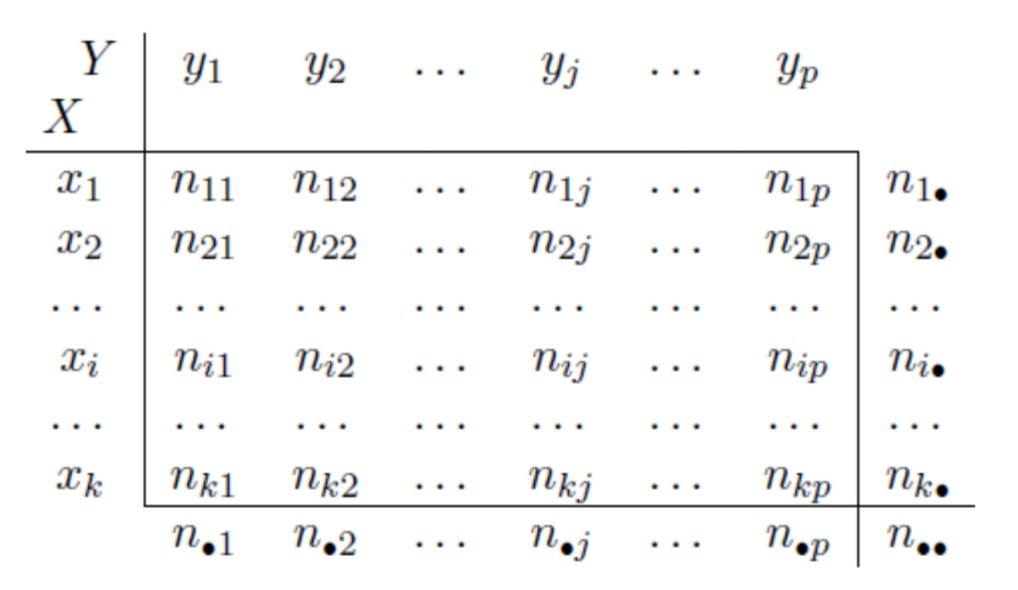
\includegraphics{./img/TablaDeContingencia.jpg} El numero de individuos
que presentan la modalida \(x_i\), es lo que llamamos \emph{frecuencia
absoluta marginal} de \(x_i\) y se representa como:

\[
\begin{array}{c}
n_{i\bullet} = n_{i1} + n_{i2} + \cdot \cdot \cdot + n_{ip} = \sum_{j=1}^p n_{ij}
\end{array}
\]

De forma análoga se define la frecuencia absoluta marginal de la
modalidad \(y_j\) como: \[
\begin{array}{c}
n_{\bullet j} = n_{1j} + n_{2j} + \cdot \cdot \cdot + n_{kj} = \sum_{i=1}^k n_{ij}
\end{array}
\] El número total de elementos de la población )o de la muestra n lo
obtenemos de cualquiera de las siguientes formas, que son equivalentes:

\[
\begin{array}{c}
n_{\bullet \bullet} = \sum_{i=1}^k n_{i \bullet} = \sum_{j=1}^p n_{ \bullet j} = \sum_{i=1}^k \sum_{j=1}^p n_{ij}
\end{array}
\]\\
\#\# Estadistico de la prueba

El estadistico de la prueba de independencia de chi-cuadrado se denota
como \(X^2\) y se calcula de la siguiente manera:

\[
\begin{array}{c}
X^2_c = \sum_{i=1}^k \sum_{j=1}^p \frac{\left( n_{ij} - \frac{n_{i \bullet} \cdot n_{\bullet j}}{n} \right)^2}{\frac{n_{i \bullet} \cdot n_{\bullet j}}{n}}
\end{array}
\] El índice \(X^2\) toma el valor de cero cuando dos variables son
independientes.

Siendo mayor que cero cuando exista asociación entre ellas, tanto mayor
cuanto más intensa sea esa correlación.

No tiene un límite máximo, lo cual supone una dificultad al nivel de
interpretarlo.

Otra forma de escribirlo es:

\[
X^2_c =\ \frac{\sum_{i =1}^{pk}  (o_i-e_i)^2}{e_i^2}\;\;\;\text{En donde}\;\;\; e_i = \frac{n_{i\bullet} \cdot n_{\bullet j}}{n_{\bullet \bullet}}
\] \#\# Ejemplo en excel

Para calcular en excel el chi cuadrado, podemos usar una tabla de
contingencia ejemplo como la siguiente:

\begin{figure}
\centering
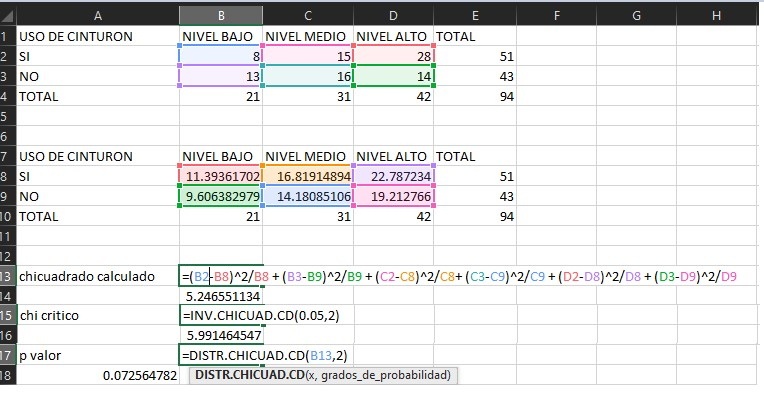
\includegraphics{./img/ejemploChiCuadrado.jpg}
\caption{}
\end{figure}

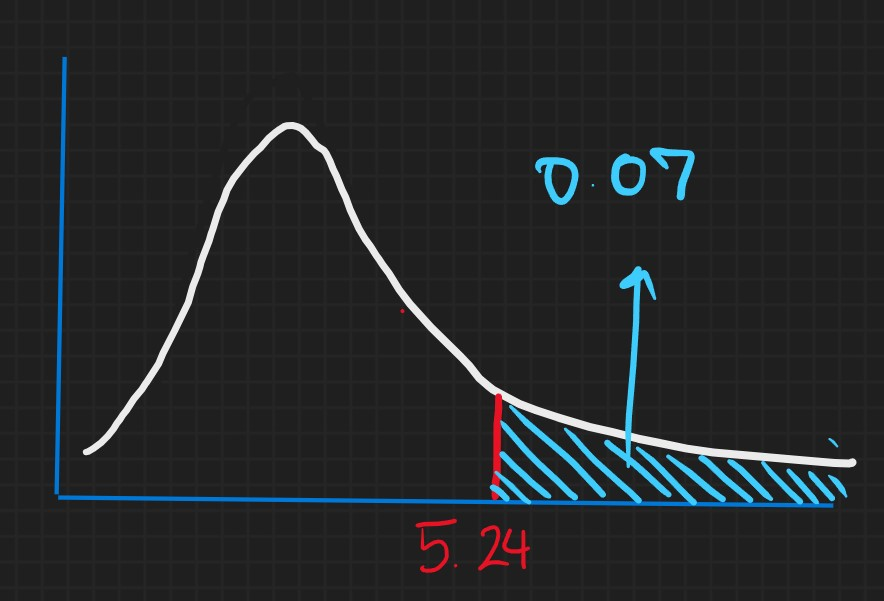
\includegraphics{./img/chiDibujo.jpg} El 7 \% de las veces que se
obtiene un valor de chi cuadrado cumpliendose la hipótesis nula, se
obtiene una suma de diferencias entre las frecuencias calculadas y las
esperadas igual o mayor al experimental. No es posible rechazar la
hipótesis nula. Es decir, la suma de las diferencias entre las
frecuencias calculadas y las esperadas no es significativamente grande
comparada con la suma de diferencias obtenida cuando la hipotesis nula
se cumple.

Entonces no es posible rechazar la hipótesis nula (En la cual no existe
asociación entre las variables). Podemos así concluir que no hay
evidencia suficiente para sugerir una asociación entre el uso de
cinturon y el nivel de escolaridad.

\begin{itemize}
\tightlist
\item
  Cuando la diferencia es pequeña, son independientes.
\item
  Cuando la diferencia es grande, están asociadas.
\end{itemize}

Podemos realizar una análigo del análisis en R.

Primero, importamos la tabla:

\begin{Shaded}
\begin{Highlighting}[]
\KeywordTok{library}\NormalTok{(readxl)}
\end{Highlighting}
\end{Shaded}

\begin{verbatim}
## Warning: package 'readxl' was built under R version 4.0.3
\end{verbatim}

\begin{Shaded}
\begin{Highlighting}[]
\NormalTok{datos <-}\StringTok{ }\KeywordTok{read_excel}\NormalTok{(}\StringTok{"./datostabla.xlsx"}\NormalTok{)}
\NormalTok{tabla <-}\StringTok{ }\KeywordTok{table}\NormalTok{(datos)}
\KeywordTok{chisq.test}\NormalTok{(tabla)}
\end{Highlighting}
\end{Shaded}

\begin{verbatim}
## Warning in chisq.test(tabla): Chi-squared approximation may be incorrect
\end{verbatim}

\begin{verbatim}
## 
##  Pearson's Chi-squared test
## 
## data:  tabla
## X-squared = 34.41, df = 6, p-value = 5.607e-06
\end{verbatim}

\texttt{Warning\ in\ chisq.test(tabla)\ :\ Chi-squared\ approximation\ may\ be\ incorrect}
Aparece proque hay celdas con frecuencias de cero. Es aconsejable hacer
la aproximación de fisher para muestras como esta.

Los grados de libertad de la prueba seria (filas-1)(columnas-1) \(\neq\)
6. Aqui quedan preguntas

\subsection{Analogo manual en R}\label{analogo-manual-en-r}

Queda pendiente para avanzar en tema, hacerlo todo manual. con ciclos
debe salir rapido

\(\phi\) \# Coeficiente \emph{phi} de pearson ()

\[
\begin{array}{c}
\phi = \sqrt{\frac{\chi^2}{n}}
\end{array}
\] Puede oscilar entre 0 y \(\sqrt{q-1}\) siendo q el mímimo número de
modalidades entre las variables (niveles).

Si \(\phi \leq 0.3\) nivel bajo de asociación Si
\(0.3 \leq \phi \leq 0.5\) nivel medio de asociación Si
\(\phi \geq 0.5\) nivel alto de asociación

Para las tablas de contingengia 2x2 oscila entre 0 y 1.

\section{Coeficiente de contingencia de
cramer}\label{coeficiente-de-contingencia-de-cramer}

\[
\begin{array}{c}
V = \sqrt{\frac{\chi^2}{n(q-1)}}
\end{array}
\]

Donde

\[
q = min[i,j]
\]

Varia entre 0 y 1.

\begin{itemize}
\tightlist
\item
  0 = independencia
\item
  Cercania a 1, intensidad de la asociacion entre las variables.
\end{itemize}

\subsection{uso en R}\label{uso-en-r}

Para calcular el coeficiente de cramer podemos usar la funcion
\texttt{cramerV} \# Coeficiente de cohen

Variable categórica dicotómica (dos niveles {[}a,b{]}) y una variable
cuantitativa Y, el índice de asociación \emph{d de cohen} se obtiene a
través de la siguiente expresión:

\[
\begin{array}{c}
d = \frac{\bar{Y}_a - \bar{Y}_b}{s_Y}
\end{array}
\]

En donde

\begin{itemize}
\tightlist
\item
  \(\bar{Y}_a\): es la media de la variable cuantitativa Y en la
  categoría a.
\item
  \(\bar{Y}_b\): es la media de la variable cuantitativa Y en la
  categoría b.
\item
  Desviación estándar de la variable \emph{Y}.
\end{itemize}

Los valores que puede tomar d no est{[}an acotados a un rango.

Pueden ser tanto positivos como negativos.

\begin{itemize}
\tightlist
\item
  d = 0, las variables son independientes.
\item
  mayor asociacion, mayor \(|d|\)
\end{itemize}

\section{El caso de dos variables
cuantitativas}\label{el-caso-de-dos-variables-cuantitativas}

\subsection{Coeficiente de correlación de
pearson}\label{coeficiente-de-correlaciuxf3n-de-pearson}

El coeficiente de correlación es la medida que describe que tan bine una
variable es explicada por otra, y se calcula:

\[
\begin{array}{c}
r_{x,y} = \frac{cov(x,y)}{\sigma_x \cdot \sigma_y} = \frac{E(xy)- E(x) \cdot E(y)}{\sigma_x \cdot \sigma_y} 
\end{array}
\] \[
\begin{array}{c}
= \frac{\frac{1}{n} \cdot \sum_{i=1}^n x \cdot y\;\; - \;\;\frac{1}{n} \cdot \sum_{i=1}^n x \cdot \frac{1}{n} \cdot \sum_{i=1}^n y }{s_x \cdot s_y}
\end{array}
\]

\[
\begin{array}{c}
-1 \leq r \leq 1
\end{array}
\]

\begin{itemize}
\tightlist
\item
  La correlacion de pearson se recomienda para variables con
  distribucion normal, para variables no normales se recomienda el uso
  de la correlacion de spearman.
\end{itemize}

\subsection{Ejemplo de correlacion}\label{ejemplo-de-correlacion}

\begin{figure}
\centering
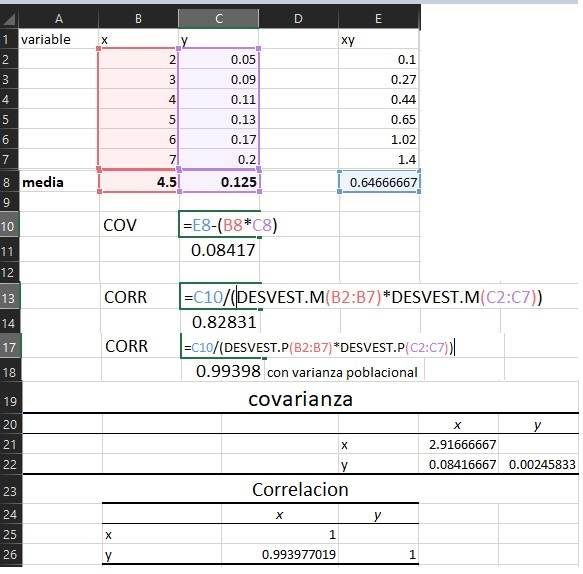
\includegraphics{./img/corrExcel.jpg}
\caption{}
\end{figure}

La imagen anterior tiene un ejemplo de como calcular la correlacion
utilizando tanto varianza muestral como poblacional. Los paquetes
estadisticos usan la varianza poblacional.

\subsection{Coeficiende de correlacion de
spearman}\label{coeficiende-de-correlacion-de-spearman}

\[
\begin{array}{c}
r_s = 1 - [6 \sum d_i^2 / (n^3-n) ] 
\end{array}
\]

Cuando se usa un estimador no parametrico, se le asigna a las
observaciones rangos.

\subsection{Ejemplo de coeficiente intelectual y horas de
TV}\label{ejemplo-de-coeficiente-intelectual-y-horas-de-tv}

Primero, se tiene el set de datos:

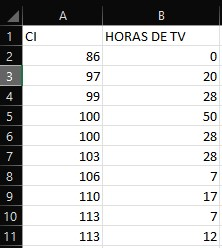
\includegraphics{./img/CI1.jpg} Luego, se le asigna un orden o un rango
a cada uno de los datos. En este caso en especial el coeficiente
intelectual (CI) ya está organizado de manera ascendente, entonces
podemos asignar un orden de la siguiente manera:

\begin{figure}
\centering
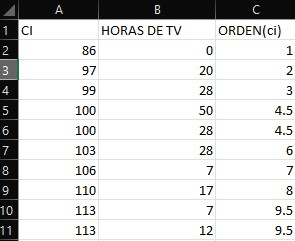
\includegraphics{./img/CI2.jpg}
\caption{}
\end{figure}

En donde el numero 100 se repote 2 veces, entonces se reparte el rango 4
y 6 entre los dos. Por esto, los dos comparten el rango promedio que es
4,5. Lo musmo sucede con el numero 113 al final, que en las dos últimas
posiciones comparte el rango 9.5, promedio de 9 y 10.

Lo mismo se puede hacer para las horas de TV:

Para este estimador se utiliza una prueba de hipótesis:

\[
\begin{array}{c}
H_0: r_s = 0 \;,\; \text{No hay correlacion}
\end{array}
\]

\[
\begin{array}{c}
H_1: r_s \neq 0 \;,\; \text{hay correlacion}
\end{array}
\]

\end{document}
